%!TEX program = xelatex
\documentclass[9pt, compress]{beamer}
\usetheme[titleprogressbar]{m}

\usepackage{array}
\usepackage{tabu}
\usepackage{longtable} %tabu needs this to be loaded.
\usepackage{lipsum}
\usepackage{multicol}
\usepackage{rotating}

\usepackage{color}
\usepackage{xcolor}
\usepackage{listings}
\usepackage{sectsty}
\usepackage{caption}


\DeclareCaptionFont{white}{\color{white}}
\DeclareCaptionFormat{listing}{\colorbox{gray}{\parbox{\dimexpr\textwidth-1.72\fboxsep\relax}{#1#2#3}}}
\captionsetup[lstlisting]{format=listing,labelfont=white,textfont=white,margin=0pt}
\lstset{language=C,
	basicstyle=\footnotesize,
	keepspaces=true,
	tabsize=4,               
	frame=single,                           % Single frame around code
	rulecolor=\color{black},
	captionpos=b,
	showstringspaces=false,	
	abovecaptionskip=-0.9pt,
	xleftmargin=3.4pt,
	xrightmargin=2.6pt,
	breaklines=true,
	postbreak=\raisebox{0ex}[0ex][0ex]{\ensuremath{\color{black}\hookrightarrow\space}},
	xleftmargin=3.2pt,
	escapechar=\&,
	literate={а}{{\selectfont\char224}}1
	{~}{{\textasciitilde}}1
	{б}{{\selectfont\char225}}1
	{в}{{\selectfont\char226}}1
	{г}{{\selectfont\char227}}1
	{д}{{\selectfont\char228}}1
	{е}{{\selectfont\char229}}1
	{ё}{{\"e}}1
	{ж}{{\selectfont\char230}}1
	{з}{{\selectfont\char231}}1
	{и}{{\selectfont\char232}}1
	{й}{{\selectfont\char233}}1
	{к}{{\selectfont\char234}}1
	{л}{{\selectfont\char235}}1
	{м}{{\selectfont\char236}}1
	{н}{{\selectfont\char237}}1
	{о}{{\selectfont\char238}}1
	{п}{{\selectfont\char239}}1
	{р}{{\selectfont\char240}}1
	{с}{{\selectfont\char241}}1
	{т}{{\selectfont\char242}}1
	{у}{{\selectfont\char243}}1
	{ф}{{\selectfont\char244}}1
	{х}{{\selectfont\char245}}1
	{ц}{{\selectfont\char246}}1
	{ч}{{\selectfont\char247}}1
	{ш}{{\selectfont\char248}}1
	{щ}{{\selectfont\char249}}1
	{ъ}{{\selectfont\char250}}1
	{ы}{{\selectfont\char251}}1
	{ь}{{\selectfont\char252}}1
	{э}{{\selectfont\char253}}1
	{ю}{{\selectfont\char254}}1
	{я}{{\selectfont\char255}}1
	{А}{{\selectfont\char192}}1
	{Б}{{\selectfont\char193}}1
	{В}{{\selectfont\char194}}1
	{Г}{{\selectfont\char195}}1
	{Д}{{\selectfont\char196}}1
	{Е}{{\selectfont\char197}}1
	{Ё}{{\"E}}1
	{Ж}{{\selectfont\char198}}1
	{З}{{\selectfont\char199}}1
	{И}{{\selectfont\char200}}1
	{Й}{{\selectfont\char201}}1
	{К}{{\selectfont\char202}}1
	{Л}{{\selectfont\char203}}1
	{М}{{\selectfont\char204}}1
	{Н}{{\selectfont\char205}}1
	{О}{{\selectfont\char206}}1
	{П}{{\selectfont\char207}}1
	{Р}{{\selectfont\char208}}1
	{С}{{\selectfont\char209}}1
	{Т}{{\selectfont\char210}}1
	{У}{{\selectfont\char211}}1
	{Ф}{{\selectfont\char212}}1
	{Х}{{\selectfont\char213}}1
	{Ц}{{\selectfont\char214}}1
	{Ч}{{\selectfont\char215}}1
	{Ш}{{\selectfont\char216}}1
	{Щ}{{\selectfont\char217}}1
	{Ъ}{{\selectfont\char218}}1
	{Ы}{{\selectfont\char219}}1
	{Ь}{{\selectfont\char220}}1
	{Э}{{\selectfont\char221}}1
	{Ю}{{\selectfont\char222}}1
	{Я}{{\selectfont\char223}}1,
	extendedchars=true
}
\usepackage{textpos}
\newcommand<>{\fullsizegraphic}[1]{
  \begin{textblock*}{0cm}(-0.9cm,-3.78cm)
  \includegraphics[width=\paperwidth]{#1}
  \end{textblock*}
}

%галочка
\usepackage{amssymb}% http://ctan.org/pkg/amssymb
\usepackage{pifont}% http://ctan.org/pkg/pifont
\newcommand{\cmark}{\ding{52}}%
\newcommand{\xmark}{\ding{56}}

\usepackage{booktabs}  
\usepackage[scale=2]{ccicons}
\usepackage{minted}
\usepgfplotslibrary{dateplot}
\usemintedstyle{trac}
\author{Студент: \textbf{Д.В. Круминьш}\\ 
	Группа: \textbf{13541/3}\\ \\
	Преподаватель: \textbf{И.А. Малышев} } 
\title{Отчет о лабораторной работе №3}
\subtitle{Курс: \textbf{Администрирование компьютерных сетей}\\
Тема: \textbf{Администрирование сетевых сервисов}}
%\logo{123}
\institute{Санкт-Петербургский политехнический университет Петра Великого}
\date{ }
%\subject{}
%\setbeamercovered{transparent}
%\setbeamertemplate{navigation symbols}{}
\begin{document}
	\maketitle
%	\begin{frame}
%		\frametitle{Оглавление}
%		\tableofcontents{}
	%\end{frame}
\begin{frame}
\frametitle{Цели работы}
\begin{enumerate}
\item Изучение состава и функциональных возможностей сетевых сервисов операционных систем.
\item Разработка и настройка сервисов локальной сети.
\item Разработка и настройка сервисов демилитаризованной зоны.
\item Разработка и настройка сервисов пограничной зоны.
\end{enumerate}
\end{frame}

\section{DHCP и удаленная загрузка}

\begin{frame}
\frametitle{Схема ККС}
Схема подверглась слующим изменениям:
\begin{enumerate}
\item К сетяи VMnet2 и VMnet3 были добавлены бездисковые клиенты;
\item В сеть VMnet3 был добавлен хост, с ОС Ubuntu;
\begin{itemize}
\item С запущенными DHCP и TFTP серверами.
\end{itemize}
\item Для сети VMnet2 в настройках VMware был отключен DHCP сервер, так как его работой займется DHCP сервер на FreeBSD.
\end{enumerate}
\end{frame}

\begin{frame}
\frametitle{Схема ККС}
\vspace*{1em}
\begin{center}
\fullsizegraphic{img/mynetwork}
\end{center}
\end{frame}

\begin{frame}[fragile]
\frametitle{Настройка DHCP на FreeBSD}
\begin{enumerate}
\item Переходим в каталог \textbf{/usr/ports/net/isc-dhcp3-server}
\item Устанавливаем следующей командой:
\begin{lstlisting}[language={}]
make install clean
\end{lstlisting}
\item Вносим в файл \textbf{/etc/rc.conf} следующие строки:
\begin{lstlisting}[language={}]
# Включаем DHCP
dhcpd_enable="YES"
# Отлючаем вывод избыточной информации
dhcpd_flags="-q" 
# Указываем интерфейс для запуска
dhcpd_ifaces="em1" 
\end{lstlisting}
\end{enumerate}
\end{frame}


\begin{frame}[fragile]
\frametitle{Настройка DHCP на FreeBSD}
\begin{enumerate}
\setcounter{enumi}{3}
\item Создаем файл \textbf{/usr/local/etc/dhcpd.conf} и вносим в него следующие изменения:
\begin{lstlisting}[language={}]
option domain-name "example.org"; # доменное имя
option domain-name-servers 192.168.32.2; #DNS сервер
default-lease-time 600; 
max-lease-time 7200; 

subnet 192.168.80.0 netmask 255.255.255.0 {
    range 192.168.80.127 192.168.80.224;
    option routers 192.168.80.2;
    option root-path "192.168.120.3:/usr/tftpboot/";
    next-server 192.168.120.3;
    filename "gpxelinux.0";
}
\end{lstlisting}
\end{enumerate}
\end{frame}


\begin{frame}[fragile]
\frametitle{Настройка Ubuntu}
Для начала необходимо корректно сконфигурировать сетеов адаптер для выхода в сеть "Интернет". Для этого были заданы следующие параметры:
\begin{itemize}
\item Адрес - 192.168.120.3;
\item Маска - 255.255.255.0;
\item Шлюз - 192.168.120.2;
\item DNS сервер - 192.168.32.2.
\end{itemize}
\end{frame}


\begin{frame}[fragile]
\frametitle{Настройка DHCP на Ubuntu}
\begin{enumerate}
\item Выполняем команду:
\begin{lstlisting}[language={}]
sudo apt-get install isc-dhcp-server
\end{lstlisting}
\item В файл \textbf{/etc/dhcp/dhcpd.conf} вносим следующие изменения:
\begin{lstlisting}[language={}]
option domain-name "example.org";
option domain-name-servers 192.168.32.2;

default-lease-time 600;
max-lease-time 7200;

subnet 192.168.120.0 netmask 255.255.255.0 {
    range 192.168.120.100 192.168.120.200;
    option routers 192.168.120.2;
    next-server 192.168.120.3;  # TFTP server address
    filename "gpxelinux.0";   # PXE boot loader filename
}
\end{lstlisting}
\item Перезапускаем DHCP-сервер
\begin{lstlisting}[language={}]
sudo /etc/init.d/isc-dhcp-server restart
\end{lstlisting}
\end{enumerate}
\end{frame}


\begin{frame}[fragile]
\frametitle{Настройка TFTP на Ubuntu}
\begin{enumerate}
\item Выполняем установку пакетов командой:
\begin{lstlisting}[language={}]
sudo apt-get install tftp tftpd-hpa
\end{lstlisting}
\item Создаем необходимые для работы директории:
\begin{lstlisting}[language={}]
mkdir -p /usr/tftpboot/images
mkdir /usr/tftpboot/pxelinux.cfg
\end{lstlisting}
\item В файл \textbf{/etc/rc.conf} вносим изменения:
\begin{lstlisting}[language={}]
tftpd_enable="YES"
tftpd_flags="-p -s /usr/tftpboot -B 1024 --ipv4"
\end{lstlisting}
\item Запускаем TFTP-сервер
\begin{lstlisting}[language={}]
service tftpd start
\end{lstlisting}
\end{enumerate}
\end{frame}


\begin{frame}[fragile]
\frametitle{Настройка TFTP на Ubuntu}
\begin{enumerate}
\setcounter{enumi}{4}
\item Скачиваем Syslinux версии 6.03 с сайта:
\begin{lstlisting}[language={}]
http://www.syslinux.org/wiki/index.php?title=The_Syslinux_Project
\end{lstlisting}
\item Извлекаем по пути \textbf{/usr/tftpboot} следующие файлы:
\begin{multicols}{2}
\begin{itemize}
\item chain.c32
\item gpxelinux.0
\item ldlinux.c32
\item libutil.c32
\item memdisk
\item menu.c32
\item reboot.c32
\item vesamenu.c32
\end{itemize}
\end{multicols}
\item Скачиваем образ ОС, поддерживающей liveCD, например ubuntu
\end{enumerate}
\end{frame}


\begin{frame}[fragile]
\frametitle{Настройка TFTP на Ubuntu}
\begin{enumerate}
\setcounter{enumi}{7}
\item Разархивируем образ ОС, по пути \textbf{/usr/tftpboot/images/ubuntu/};
\item По пути \textbf{/usr/tftpboot/pxelinux.cfg} создаем файл \textbf{default} со следующим содержимым:
\begin{lstlisting}[language={}]
ui menu.c32
menu title Netboot OS

LABEL ubuntu
        kernel images/ubuntu/casper/vmlinuz.efi
        append root=/dev/nfs boot=casper netboot=nfs nfsroot=192.168.120.3:/usr/tftpboot/images/ubuntu initrd=images/ubuntu/casper/initrd.lz 
\end{lstlisting}
\item Перезгружаем ОС.
\end{enumerate}
\end{frame}


\begin{frame}[fragile]
\frametitle{Запуск бездисковых клиентов}
Запускаем бездисковые клиенты. При запуске вспывет меню, с выбором дальнейшей загрузки.
\begin{center}  
	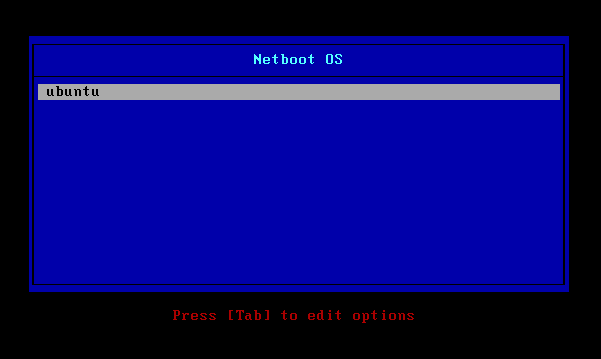
\includegraphics[width=\textwidth]{img/nodisk}
\end{center}
\end{frame}


\begin{frame}[fragile]
\frametitle{Бездисковый клиент сети VMnet3}
\begin{center}  
	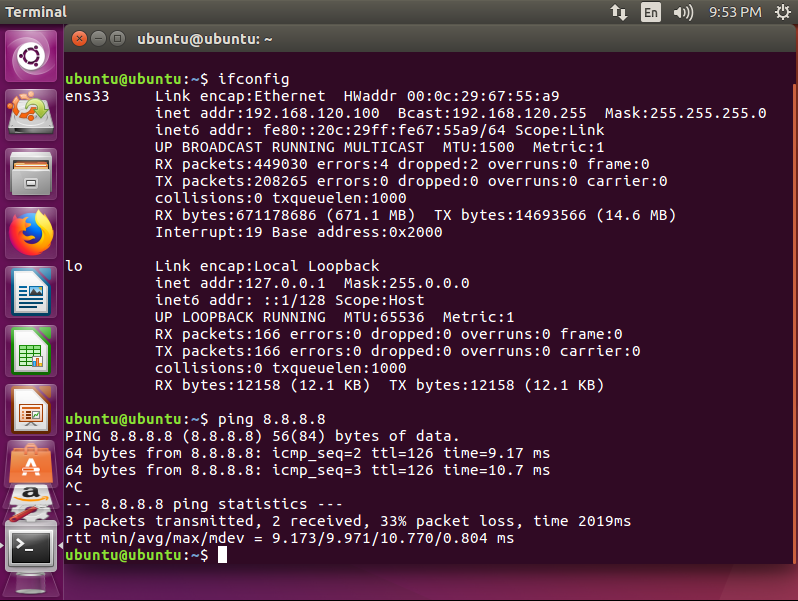
\includegraphics[width=.9\textwidth]{img/nodisk1_1}
\end{center}
\end{frame}


\begin{frame}[fragile]
\frametitle{Бездисковый клиент сети VMnet2}
\begin{center}  
	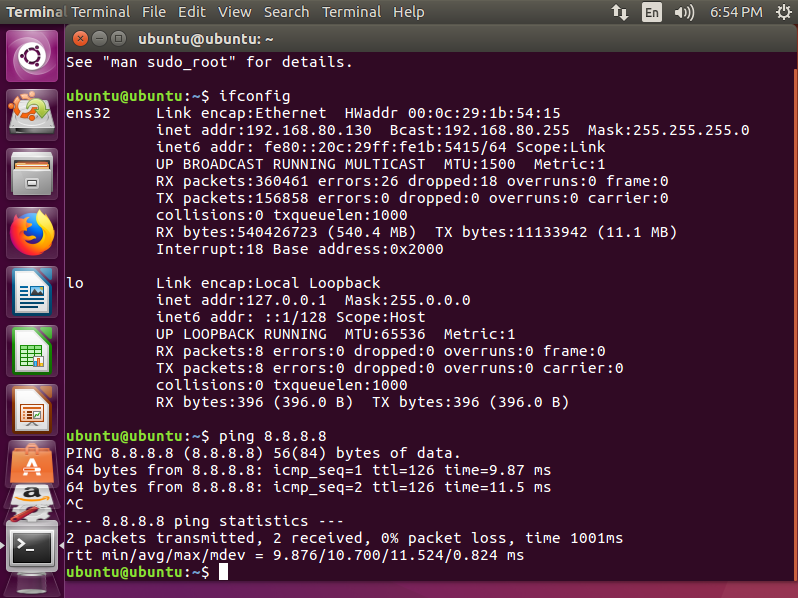
\includegraphics[width=.9\textwidth]{img/nodisk2_1}
\end{center}
\end{frame}


\begin{frame}[fragile]
\frametitle{Итог работы бездисковых клиентов}
Как видно из результатов, клиенты посредством двух разных DHCP сервером успешно получили адреса, а также подключились к TFTP-серверу, вследствии чего была выполнена удаленная загрузка.
\end{frame}

\section{DNS сервисы}

\begin{frame}
\frametitle{Настройка DNS сервера}
В данном разделе будут приведены примеры различных DNS серверов, в частности:
\begin{enumerate}
\item \textbf{Кэширующий сервер} - ищет все ответы на запросы от пользователей и запоминает их на случай повторного запроса
\item \textbf{Первичный мастер} - читает данные зоны из локального файла и является ответственным за эту зону
\item \textbf{Вторичный мастер} - получает данные по зоне с другого сервера имен,
отвечающего за эту зону
\end{enumerate}
В схеме ККС также будет использоваться Linux Mint(192.168.40.32).
\end{frame}


\begin{frame}
\frametitle{Схема ККС}
\vspace*{1em}
\begin{center}
\fullsizegraphic{img/mynetwork2}
\end{center}
\end{frame}


\begin{frame}[fragile]
\frametitle{Настройка кэширующего сервера}
Установим кэширующий DNS на Linux Mint(192.168.40.32)
\begin{enumerate}
\item Устанавливаем пакет \textbf{bind} командой
\begin{lstlisting}[language={}]
sudo apt-get install bind9
\end{lstlisting}
\item Внесем изменения в файл \textbf{/etc/bind/named.conf.options}:
\begin{lstlisting}[language={}]
options {
  directory "/var/cache/bind";
  forwarders {
    8.8.8.8;
  };
  dnssec-validation auto;
  auth-nxdomain no;
  listen-on-v6 {any;};
};
\end{lstlisting}
\item Перезапускаем DNS сервер
\begin{lstlisting}[language={}]
sudo /etc/init.d/bind9 restart
\end{lstlisting}
\end{enumerate}
\end{frame}


\begin{frame}[fragile]
\frametitle{Проверка кэширующего сервера}
\begin{enumerate}
\item Настроим хост \textbf{192.168.120.3} на использование данного DNS сервера;
\item В файле \textbf{/etc/NetworkManager/NetworkManager.conf} комментируем строку \textbf{dns=dnsmasq}, иначе в nslookup будет другой адрес DNS;
\item Перезагружаем систему;
\item Вводим команду \textbf{nslookup ya.ru}, после чего в консоль будет выведено:
\begin{lstlisting}[language={}]
Server:        192.168.40.32
Address:       192.168.40.32#53

Non-authoritative answer:
Name:    ya.ru
Address: 87.250.250.242
\end{lstlisting}
Как видно, DNS успешно был определен.
\end{enumerate}
\end{frame}


\begin{frame}[fragile]
\frametitle{Проверка кэширующего сервера}
Дополнитьно проверим кэширующую способность DNS сервера, для этого введем команду \textbf{dig google.com} два раза:
\begin{lstlisting}[language={}]
dig google.com
...
;; Query time: 31 msec
;; SERVER: 192.168.40.32#53(192.168.40.32)
;; WHEN: Fri Mar 23 11:55:03 PDT 2018
;; MSG SIZE  rcvd: 346


dig google.com
...
;; Query time: 0 msec
;; SERVER: 192.168.40.32#53(192.168.40.32)
;; WHEN: Fri Mar 23 11:55:03 PDT 2018
;; MSG SIZE  rcvd: 346
\end{lstlisting}
Как видно, время запроса снизилось с 32 до 0 милисекунд, что означает о наличии кэширующей возможности у DNS сервера.
\end{frame}


\begin{frame}[fragile]
\frametitle{Настройка первичного DNS сервера}
Первичный сервер - \textbf{192.168.40.32}, вторичный - \textbf{192.168.120.3}.
\begin{enumerate}
\item В файл \textbf{/etc/bind/named.conf.local} вносим изменения:
\begin{lstlisting}[language={}]
zone "example.com" {
  type master;
  file "/etc/bind/db.example.com";
  allow-transfer {192.168.40.0/24;192.168.80.0/24;192.168.120.0/24;};
};
zone "40.168.192.in-addr.arpa" {
  type master;
  file "/etc/bind/db.192";
  allow-transfer {192.168.40.0/24;192.168.80.0/24;192.168.120.0/24;};
}; 
\end{lstlisting}
\end{enumerate}
Были созданы зоны \textbf{example.com} и обратная ей зона(для получения имени по IP)
\end{frame}


\begin{frame}[fragile]
\frametitle{Настройка первичного DNS сервера}
Содержимое файла \textbf{db.example.com} выглядит следующим образом:
\begin{lstlisting}[language={}]
;
; BIND data file for example.com
;
$TTL    604800
@   IN   SOA   example.com. root.example.com. (
             1          ; Serial
             604800     ; Refresh
              86400     ; Retry
            2419200     ; Expire
             604800 )   ; Negative Cache TTL
    IN A   192.168.40.32
;
@   IN  NS  ns.example.com
@   IN  A  192.168.40.32
@   IN  AAAA    ::1
ns  IN  A  192.168.40.32
\end{lstlisting}
\end{frame}


\begin{frame}[fragile]
\frametitle{Настройка первичного DNS сервера}
Содержимое файла \textbf{db.192} выглядит следующим образом:
\begin{lstlisting}[language={}]
;
; BIND reverse data file for local 192.168.40.XXX net
;
$TTL    604800
@       IN      SOA     ns.example.com. root.example.com. (
                         1              ; Serial
                         604800         ; Refresh
                          86400         ; Retry
                        2419200         ; Expire
                         604800 )       ; Negative Cache TTL
;
@       IN      NS      ns.
32      IN      PTR     ns.example.com.
\end{lstlisting}
В данном случае адресу 192.168.40.32 соответствует имя example.com. 
\end{frame}


\begin{frame}[fragile]
\frametitle{Настройка вторичного DNS сервера}
\begin{enumerate}
\item Устанавливаем пакет bind9;
\item В файл \textbf{/etc/bind/named.conf.local} вносим изменения:
\begin{lstlisting}[language={}]
zone "example.com" {
  type slave;
  file "db.example.com";
  masters { 192.168.40.32; };
};        
zone "40.168.192.in-addr.arpa" {
  type slave;
  file "db.192";
  masters { 192.168.40.32; };
};
\end{lstlisting}
\end{enumerate}
Теперь данный сервер является вторичным по отношению к 192.168.40.32.
\end{frame}


\begin{frame}[fragile]
\frametitle{Проверка первичного и вторичного DNS сервером}
На первичном сервере вводим команду \textbf{cat /etc/log/syslog}
\begin{lstlisting}[language={}]
...
... zone example.com/IN: loaded serial 1
... zone 40.168.192.in-addr.arpa/IN: loaded serial 1
... zone 255.in-addr.arpa/IN: loaded serial 1
... zone localhost/IN: loaded serial 2
... all zones loaded
... running
... zone 40.168.192.in-addr.arpa/IN: sending notifies (serial 1)
...
\end{lstlisting}
Как видно из части лога, зоны были успешно загружены и переданы на вторичный сервер.
\end{frame}


\begin{frame}[fragile]
\frametitle{Вывод}
В данной работе был получен опыт по настройке DHCP и TFTP серверов, что позволяет загружать по сети ОС или утилиту. 

Также были применены навыки работы с различными по функциональности DNS серверами. Так был получен кэширующий DNS сервер, который существенно ускоряет обращение к сетевым ресурсам. Также были сконфигурированы первичный и вторичный DNS сервера, ответственные за домен example.com и обратную зону.
\end{frame}	
	

	
\end{document}
